%%%%%%%%%%%%%%%%%%%%%%%%%%%%%%%%%%%%%%%%%
% Journal Article
% LaTeX Template
% Version 1.1 (25/11/12)
%
% This template has been downloaded from:
% http://www.LaTeXTemplates.com
%
% Original author:
% Frits Wenneker (http://www.howtotex.com)
%
% License:
% CC BY-NC-SA 3.0 (http://creativecommons.org/licenses/by-nc-sa/3.0/)
%
%%%%%%%%%%%%%%%%%%%%%%%%%%%%%%%%%%%%%%%%%

%----------------------------------------------------------------------------------------
%	PACKAGES AND OTHER DOCUMENT CONFIGURATIONS
%----------------------------------------------------------------------------------------

\documentclass[twoside]{article}

\usepackage{amsmath}
\usepackage{graphicx}
\usepackage{lipsum} % Package to generate dummy text throughout this template

\usepackage[sc]{mathpazo} % Use the Palatino font
\usepackage[T1]{fontenc} % Use 8-bit encoding that has 256 glyphs
\linespread{1.05} % Line spacing - Palatino needs more space between lines
\usepackage{microtype} % Slightly tweak font spacing for aesthetics

\usepackage[hmarginratio=1:1,top=32mm,columnsep=20pt]{geometry} % Document margins
\usepackage{multicol} % Used for the two-column layout of the document
\usepackage{hyperref} % For hyperlinks in the PDF

\usepackage[hang, small,labelfont=bf,up,textfont=it,up]{caption} % Custom captions under/above floats in tables or figures
\usepackage{booktabs} % Horizontal rules in tables
\usepackage{float} % Required for tables and figures in the multi-column environment - they need to be placed in specific locations with the [H] (e.g. \begin{table}[H])

\usepackage{lettrine} % The lettrine is the first enlarged letter at the beginning of the text
\usepackage{paralist} % Used for the compactitem environment which makes bullet points with less space between them

\usepackage{abstract} % Allows abstract customization
\renewcommand{\abstractnamefont}{\normalfont\bfseries} % Set the "Abstract" text to bold
\renewcommand{\abstracttextfont}{\normalfont\small\itshape} % Set the abstract itself to small italic text

\usepackage{fixltx2e}
\usepackage{caption}
%\usepackage{subcaption}

\usepackage{titlesec} % Allows customization of titles
\renewcommand\thesection{\Roman{section}}
\titleformat{\section}[block]{\large\scshape\centering}{\thesection.}{1em}{} % Change the look of the section titles
%----------------------------------------------------------------------------------------
%	TITLE SECTION
%----------------------------------------------------------------------------------------

\title{\vspace{-15mm}\fontsize{14pt}{12pt}\selectfont\textbf{Predictinig Parkinson's Disease Utilizing Support Vector Machines using Audio Features}} % Article title

\author{
\large
\textsc{Robert Micatka}\\ % Your name
\normalsize University of Michigan \\ % Your institution
}


%----------------------------------------------------------------------------------------

\makeatletter
\newenvironment{tablehere}
  {\def\@captype{table}}
  {}

\newenvironment{figurehere}
  {\def\@captype{figure}}
  {}
\makeatother


\begin{document}


\maketitle 

\date{}

%----------------------------------------------------------------------------------------
%	ABSTRACT
%----------------------------------------------------------------------------------------

\begin{abstract}

	Parkinson's disease is a prevalent chronic neurological disease that can be recognized by the severe
motor system disorders that it causes. An early detection system would be beneficial to diagnose people
early in order to maximize their quality of life. A system was created that utilizes exclusively audio
data which allows for lightweight implementations to be created on such platforms as smartphones and personal computers.
 
\end{abstract}

%----------------------------------------------------------------------------------------
%	ARTICLE CONTENTS
%----------------------------------------------------------------------------------------

\begin{multicols}{2} % Two-column layout throughout the main article text

\section{Introduction}

\lettrine[nindent=0em,lines=3]{P} arkinson's disease is a debilitating and neurological disorder that is manifested primarily
through motor system disorders but later on in the disease progression psychiatric symptoms such as
dementia and depression can occur. One million Americans and 7-10 million worldwide are affected by
this disease with approximately 60,000 new diagnoses every year (in the United States). This is more
than the combined number of people affected by multiple sclerosis, muscular dystrophy and Lou
Gehrig's disease. Diagnosis of this disease is a growing research area as it can be difficult to distinguish
Parkinson's from other neurological diseases such as Alzheimer's.
There is currently no cure for Parkinson's disease, however there are many treatments that a patient can receive
that will drastically improve the quality of life. Therefore early detection of this disease is crucial to
help patients until a cure is found.\\
Previous research has been done in order to design systems for early detection but have relied exclusively 
on accelerometer and similar data. This is a logical choice when examining Parkinson's but is limited
in the ease of implementing this system at wide scales. An audio-based system would be preferred for early
detection as it can be easily implemented on a variety of platforms.

\section{Data}

The Michael J. Fox Foundation for Parkinson's Research has collected and opened up a large
database of mobile phone data collected from healthy adults as well as those with different stages of
Parkinson's. Using mobile phone data which uses a variety of sensors to collect data could lead to early
detection of this disease as it primarily manifests through motor system disorders which can be
registered through speech and motor patterns. The data contains data from audio, accelerometry,
compass, ambient light, proximity, battery level and GPS streams. The data was recorded every minute
in one hour increments during waking hours. The study lasted for 8 weeks. There were 16 participants in the study,
9 diagnosed with Parkinson's and 7 controls.\\
This dataset has been analyzed in the past but the focus was on the accelerometry and GPS data. 
This project is looking exclusively at the audio data as it has not been examined in the past. 
The audio data provided contains several features such as L1-norm, L2-norm, L-inf norm,
power spectral density across four separate bands, 12 lowest mel-frequency cepstral coefficients.
The data was provided in csv format and seperated by subject and day.
Due to the vast amount of data (on the order of 200,000 data-points) the data was averaged over each day (for
each subject). This reduces the data to a manageable level in order to be used for machine learning.


%------------------------------------------------

\section{Methods}

In order to classify data into Parkinson's or not Parkinson's a support vector machine was utilized.
This machine learning technique is ideal for this type of problem because it is simply a binary 
classification. Support vector machines work by projecting the training data into a higher dimension in 
order to seperate it using a hyperplane. The hyperplane is defined as follows:\\ 
$f(x) = w^T \phi (x) + b$\\ \\
where $w$ is the margin or seperation between the two classes and $f(x)>0$ implies $y = 1$
and $f(x) <0$ implies $y = -1$ and $x$ and $y$ are the two classes.\\ 
To create good seperation the support vector machine attempts to maximize
the margin. This is achieved by using Lagrange multipliers as shown in the following equation.\\ 
$L(w,b,a) = \frac{1}{2} || w||^2 - \sum \limits_{n=1} ^{N} \alpha_n [ y_n (w \cdot x_n -b) -1 ] $\\
Support vector machines rely on the kernel in order to seperate the data after it has been projected. There are many
different types of kernels that perform differently depending on the dataset. Common kernels include linear, quadratic,
other polynomials and radial basis functions. Only linear and radial basis functions were examined as kernels in
this project.
Support vector machines work well if there is not miss-classified data or
outliers. However, outlying data points can make it extremely difficult for support vector machines to find
the correct seperating hyperplane. The support vector machine may not find the hyperplane at all as it has to project
to such a high dimension that computational resources are exhausted. Another, potentially more serious, problem
is that a hyperplane may be found but overfits the data, it is so complicated that it is useless when classifying testing data.
In order to alleviate this problem a "soft margin" term can be used which allows for outliers in the
data (but penalizes them). This is implemented by using the following equation:\\ 
$C \sum \limits_{n=1} ^{N} \xi _n + \frac{1}{2} || w ||^2$\\ \\
In order to maximize the available data, and to prevent overfitting, $k$-folds cross-validation is used.
This technique seperates the data in $k-1$ training samples and $k$ testing samples. This process is
repeated $k$ times in order for all of the available data to be used for both training and testing.\\
The data was first imported into MATLAB and averaged over each day in order to reduce the number of observations
to allow the support vector machine to function better. The data was seperated into three
different matrices, the power spectral density values, the energy values, and the Mel-frequency cepstral coefficients.
These were the different features used to train and test the support vector machines.
Two different groups were created, those with Parkinson's disease (positive)
and the controls (negative). 10-fold cross-validation was implemented using a MATLAB function that
provided indices. The support vector machine used for the classification was implemented using MATLAB
and then tuned using parameter sweeping over possible soft margin values and either linear or radial basis function
kernels. The rates for each pass of the cross-validation were weighted appropriately and summed to get
an overall rate.

%------------------------------------------------





\section{Results}

The classification rates when examining the Power Spectral Density feature
compared to the soft margin parameter when using a linear kernel is as follows:\\ \\
\begin{tabular}{|c|c|c|}
	\hline
	Soft Margin 	& Positive Rate & Negative Rate \\ \hline
	0.1		& 0.9378	& 0.3216 \\ \hline
	0.2		& 0.9270	& 0.3351 \\ \hline
	0.3		& 0.9135	& 0.3405 \\ \hline
	0.4		& 0.9081	& 0.3486\\ \hline
	0.5		& 0.8973	& 0.3649\\ \hline
	0.6		& 0.9000	& 0.3757\\ \hline
	0.7		& 0.8919	& 0.3676\\ \hline
	0.8		& 0.8892	& 0.3757\\ \hline
	0.9		& 0.8811	& 0.3865\\ \hline
	1.0		& 0.8892	& 0.3811 \\ \hline
\end{tabular}

The classification rates when examining the Power Spectral Density feature
compared to the soft margin parameter when using a radial basis function kernel is as follows:\\ \\
\begin{tabular}{|c|c|c|}
	\hline
	Soft Margin 	& Positive Rate & Negative Rate \\ \hline
	0.1		& 0.8919	& 0.3514 \\ \hline
	0.2		& 0.8197	& 0.4554 \\ \hline
	0.3		& 0.8468	& 0.4635 \\ \hline
	0.4		& 0.8487	& 0.4702\\ \hline
	0.5		& 0.8541	& 0.4720\\ \hline
	0.6		& 0.8611	& 0.4810\\ \hline
	0.7		& 0.8557	& 0.4953\\ \hline
	0.8		& 0.8522	& 0.4957\\ \hline
	0.9		& 0.8649	& 0.4918\\ \hline
	1.0		& 0.8630	& 0.5008 \\ \hline
\end{tabular}



\vfill
\columnbreak



The classification rates when examining the energy feature
compared to the soft margin parameter when using a linear kernel is as follows:\\ \\
\begin{tabular}{|c|c|c|}
	\hline
	Soft Margin 	& Positive Rate & Negative Rate \\ \hline
	0.1		& 0.6360	& 0.6197 \\ \hline
	0.2		& 0.6719	& 0.6090 \\ \hline
	0.3		& 0.6936	& 0.6072 \\ \hline
	0.4		& 0.6936	& 0.6035\\ \hline
	0.5		& 0.6902	& 0.6123\\ \hline
	0.6		& 0.6920	& 0.6145\\ \hline
	0.7		& 0.6881	& 0.6181\\ \hline
	0.8		& 0.6885	& 0.6163\\ \hline
	0.9		& 0.6902	& 0.6269\\ \hline
	1.0		& 0.6881	& 0.6144 \\ \hline
\end{tabular}




The classification rates when examining the energy feature
compared to the soft margin parameter when using a radial basis kernel is as follows:\\ \\
\begin{tabular}{|c|c|c|}
	\hline
	Soft Margin 	& Positive Rate & Negative Rate \\ \hline
	0.1		& 0.7907	& 0.4761 \\ \hline
	0.2		& 0.7765	& 0.4776 \\ \hline
	0.3		& 0.7801	& 0.4921 \\ \hline
	0.4		& 0.7820	& 0.4917\\ \hline
	0.5		& 0.7857	& 0.4953\\ \hline
	0.6		& 0.7785	& 0.4993\\ \hline
	0.7		& 0.7838	& 0.4972\\ \hline
	0.8		& 0.7782	& 0.5066\\ \hline
	0.9		& 0.7819	& 0.5007\\ \hline
	1.0		& 0.7804	& 0.5079 \\ \hline
\end{tabular}

\newpage
The classification rates when examining the Mel-frequency cepstrum coefficients feature
compared to the soft margin parameter when using a linear kernel is as follows:\\ \\
\begin{tabular}{|c|c|c|}
	\hline
	Soft Margin 	& Positive Rate & Negative Rate \\ \hline
	0.1		& 0.8167	& 0.7512 \\ \hline
	0.2		& 0.8158	& 0.7623 \\ \hline
	0.3		& 0.8225	& 0.7784 \\ \hline
	0.4		& 0.8099	& 0.7678\\ \hline
	0.5		& 0.0	& 0.0\\ \hline
	0.6		& 0.0 	& 0.0\\ \hline
	0.7		& 0.0 	& 0.0\\ \hline
	0.8		& 0.0 	& 0.0\\ \hline
	0.9		& 0.0	& 0.0\\ \hline
	1.0		& 0.0	& 0.0 \\ \hline
\end{tabular}
The classification rates when examining the Mel-frequency cepstrum coefficients feature
compared to the soft margin parameter when using a radial basis kernel is as follows:\\ \\
\begin{tabular}{|c|c|c|}
	\hline
	Soft Margin 	& Positive Rate & Negative Rate \\ \hline
	0.1		& 0.8774	& 0.7477 \\ \hline
	0.2		& 0.9079	& 0.7670 \\ \hline
	0.3		& 0.9295	& 0.7944 \\ \hline
	0.4		& 0.9301	& 0.8006\\ \hline
	0.5		& 0.9076	& 0.8287\\ \hline
	0.6		& 0.9026	& 0.8327\\ \hline
	0.7		& 0.9196	& 0.8488\\ \hline
	0.8		& 0.9082	& 0.8596\\ \hline
	0.9		& 0.9129	& 0.8602\\ \hline
	1.0		& 0.9187	& 0.8421 \\ \hline
\end{tabular}

\end{multicols}

A graph of each feature after parameter optimization using both kernels is as follows:\\
\begin{center}
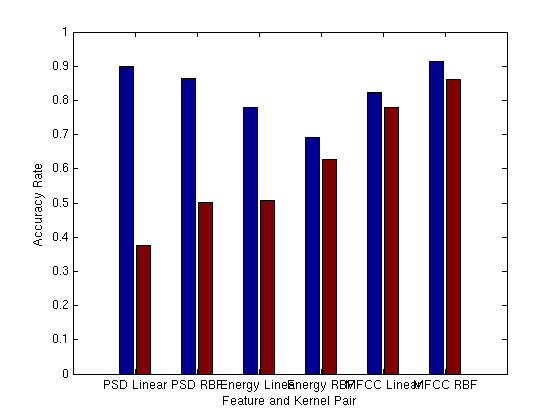
\includegraphics[scale=0.9]{accuracy_rates.png}
\end{center}
%------------------------------------------------

\newpage
\begin{multicols}{2}

\section{Discussion and Further Study}

As seen in the results the overall accuracy rates were quite varied, some features
performed quite well while others did poorly. The power-spectral-density had a high positive
accuracy rate but an extremely low negative accuracy rate for both the linear and the radial
basis function kernels. The energy feature had better negative accuracy rates but low 
positive accuracy rates. The energy feature had a stark difference when using the linear
kernel compared to the radial basis kernel for negative accuracy rates. The Mel-frequency cepstrum
coefficients had the best classification rates, a respectable 91\% positive rate and 86\%
negative rate. This is quite good and shows promise for further study.\\
Overall the data did show good positive classification rates when using the Mel-frequency cepstrum
coefficients as well as the power spectal density features. However, the power-spectral density feature had
quite low negative classification rates. This is not acceptable when making a real-world system
as false-negatives should be minimized, people should not be told they are not at risk for Parkinson's
when they are. This contrasts to false-positives where people are told they might have Parkinson's and
then do not. This type of error is acceptable as it is easy to catch with further testing while
false-negatives are not.\\
A better classification system could potentially be developed that combined the three
feature types together and weighted them appropriately. The audio data classification system could
also be combined with an accelerometer based system in order to increase accuracy. In addition, while 
outside of the available dataset other audio features could be examined. Raw audio was not available
when developing this system but different audio data could be collected and analyzed in the future.



\end{multicols}





\end{document}
